%
% CHAPTER 6.- The Theory of Nescience
%

\chapterimage{owl.pdf} % Chapter heading image

\chapter{Nescience}
\label{chap:Nescience}

\begin{quote}
\begin{flushright}
\emph{There are known knowns. These are things we know that we know.
There are known unknowns. That is to say, there are things that we know we don't know.
But there are also unknown unknowns. There are things we don't know we don't know.} \\
Donald Rumsfeld
\end{flushright}
\end{quote}
\bigskip

Following the foundational Chapter \ref{cha:Topics-and-Descriptions}, which introduced the core concepts of entity, representation, and description, and the subsequent Chapters \ref{chap:Miscoding}, \ref{chap:Error}, and \ref{chap:Redundancy}, which developed the new metrics of miscoding, inaccuracy, and surfeit, we are now prepared to delve into the central concept of nescience in this chapter, focusing on its fundamental properties.

Unlike Shannon entropy or Kolmogorov complexity, which measure information, nescience quantifies the absence of information, that is, what remains unknown. The theory of nescience characterizes our ignorance about a research entity through the three previously introduced metrics: miscoding, inaccuracy, and surfeit. Miscoding assesses how accurately an entity is represented as a string of symbols; inaccuracy measures how well our best available model describes this representation; and surfeit evaluates the descriptive efficiency of the model, as reflected in its length or symbol count.

These three metrics are inherently interdependent and often in conflict: reducing one can lead to an increase in another. The central challenge, therefore, is to develop a method for simultaneously minimizing all three. This requirement reflects, in our view, the fundamental nature of scientific inquiry as a multi-objective optimization problem.

One of the most significant outcomes of our definition of nescience, grounded in the metrics of miscoding, inaccuracy, and surfeit, is its capacity to partition the domain of research topics into two distinct areas. The first is the known unknown, which includes topics we are aware we do not fully understand, yet can recognize and acknowledge our incomplete knowledge. The second is the unknown unknown, comprising topics that have not yet been discovered or conceptualized. A key application of the theory of nescience is its use as a methodological framework for identifying and exploring what lies within the unknown unknown.

Another noteworthy implication of the nescience framework is the counterintuitive idea that, for certain topics, continued research may be counterproductive. In these cases, additional investigation may actually increase our ignorance rather than reduce it. This occurs when we reach a critical threshold beyond which our descriptions become more inaccurate, overly complex, or based on flawed representations, preventing any real progress toward understanding. 

%
% Section: Nescience
%

\section{Nescience}

Intuitively, our understanding of an entity should be based in the quality of the model we use to describe it, specifically, its ability to explain why things happen. Within the theory of nescience, we propose a quantitative measure of our ignorance concerning a research entity, based on three components: the miscoding of a string-based representation of the entity, and the inaccuracy and surfeit of the model describing that representation. Miscoding captures how accurately the representation encodes the entity, inaccuracy reflects how well the model describes the representation, and surfeit quantifies the extent of unnecessary effort embedded in the model. We argue that the goal of science should be to minimize all three quantities: miscoding, inaccuracy, and surfeit. Unfortunately, these metrics are inherently conflicting, reducing one may lead to an increase in one or both of the others.

According to the theory of nescience, science can be viewed as a multiobjective optimization problem\footnote{Technically speaking, science is a deterministic, discrete, nonlinear, nonconvex, nondifferentiable multiobjective optimization problem with a single decision maker.} (see Section \ref{sec:multiobjective_optimization}):

\begin{tBox}
\textbf{The Science Problem}
\index{Sicence problem}
\begin{align*}
 & \text{minimize} \quad \{ \mu(r), \iota(d, r), \sigma(d, r)\} \\
 & \text{subject to} \quad (r, d) \in \mathcal{B}^\ast \times \mathcal{D}
\end{align*}
\end{tBox}

A \emph{scientific method}\index{Scientific method}, further discussed in Chapter \ref{chap:Philosophy}, refers to any algorithm or computable procedure capable of solving, or closely approximating a solution to, the above minimization problem. This includes a broad class of techniques and methodologies aimed at systematically reducing the values of miscoding, inaccuracy, and surfeit. In doing so, scientific methods contribute to improving the accuracy and conciseness of our representations and models, thereby advancing our understanding of the world.

The feasible region is the Cartesian product $\mathcal{B}^\ast \times \mathcal{D}$, where $\mathcal{B}^\ast$ denotes the set of finite binary strings and $\mathcal{D}$ the set of descriptions. The decision vectors are pairs $(r, d)$, referred to as \emph{hypotheses}\index{Hypothesis}, consisting of a representation and a description. The objective functions to be minimized are miscoding, surfeit, and inaccuracy. The objective space is the subset $\mathbf{Z} \subset \mathbb{R}^3$, whose elements are the objective vectors.

In our formulation of science and the scientific method, we deliberately exclude the set $\mathcal{E}$ of entities. Requiring direct knowledge of an entity $e \in \mathcal{E}$ would render the scientific problem ill-posed for most research areas. Science, at its core, is a matter of manipulating strings of symbols. From a practical standpoint, it is about discovering strings that have meaningful interpretations in the real world and can be used to solve concrete problems. From a more theoretical perspective, the aim of science can be seen as the attempt to understand the workings of an unknown abstract oracle.

If the set $\mathcal{R}_e$ of representations for a particular entity $e$ is known, or approximately known, we can restrict the science problem to:
\begin{align*}
 & \text{minimize} \quad \{ \mu(r), \iota(d, r), \sigma(d, r)\} \\
 & \text{subject to} \quad (r, d) \in \mathcal{R}_e \times \mathcal{D}
\end{align*}
Within the theory of nescience, our primary focus lies in the decision space $\mathcal{B}^\ast \times \mathcal{D}$, the space of representations and descriptions, rather than in the objective space $\mathbf{Z} \subset \mathbb{R}^3$ of metric values. In the following definitions, we revisit key concepts from multiobjective optimization (see Section \ref{sec:multiobjective_optimization}) as they apply specifically to the science problem.

\subsection*{Pareto Optimality}

If the representation and description currently used to characterize an entity are not perfect, our goal is to find an alternative representation or description that reduces at least one of the metrics miscoding, inaccuracy, or surfeit without increasing the value of any of the others.

\begin{definition}
We say that a hypothesis $(r, d) \in \mathcal{B}^\ast \times \mathcal{D}$ \emph{dominates}\index{Dominate} another hypothesis $(r', d') \in \mathcal{B}^\ast \times \mathcal{D}$ if it improves at least one of the metrics miscoding, inaccuracy, or surfeit without worsening either of the other two.
\end{definition}

For example, we might identify a new representation that encodes the entity more accurately without degrading the quality of its description. Alternatively, we could find a new description that improves accuracy without increasing surfeit, or a more concise description that preserves accuracy.

\begin{example}
\label{ex:nescience_pareto}
Consider an experiment in which we collect a set of observations $r$ and apply a mathematical model $f_1$ from a model family $\mathcal{M}_1$, resulting in an inaccuracy of $i_1$. Later, we fit a second model $f_2$ from a different model family $\mathcal{M}_2$, which is smaller in size (i.e., has lower surfeit) but yields the same inaccuracy $i_1$. In this case, the hypothesis $B = (r, f_2)$ dominates the hypothesis $A = (r, f_1)$, even though it is not better in terms of inaccuracy alone.
\end{example}

For most entities, there does not exist a single solution that simultaneously minimizes all three metrics. Instead, we encounter a set of Pareto optimal solutions that define an optimal frontier.

\begin{definition}
We say that a hypothesis $(r, d) \in \mathcal{B}^\ast \times \mathcal{D}$ is \emph{Pareto optimal}\index{Pareto optimal} if there does not exist another hypothesis $(r', d') \in \mathcal{B}^\ast \times \mathcal{D}$ such that $(r', d')$ dominates $(r, d)$. The set of Pareto optimal solutions, denoted by $\mathbf{P}_{\mathcal{B}^\ast \times \mathcal{D}}$, is called the \emph{Pareto frontier}\index{Pareto frontier}.
\end{definition}

In the realm of scientific research, the concept of the Pareto frontier, as defined by the set of Pareto optimal solutions $\mathbf{P}_{\mathcal{B}^\ast \times \mathcal{D}}$, plays a crucial role. It delineates the boundary of optimal trade-offs among the conflicting metrics of miscoding, inaccuracy, and surfeit, such that none can be improved without worsening at least one of the others. This frontier represents the spectrum of best-achievable balances, guiding researchers to identify models and representations that offer the most scientifically rigorous understanding of their subject matter (see Section \ref{sec:perfect_knowledge}).

However, in certain situations or specific applications, it may be reasonable to adopt a solution that is not Pareto optimal. For instance, one might choose to prioritize a particular metric due to its relevance or importance to the research objectives, accepting less favorable values for the remaining metrics as a necessary trade-off (see Section \ref{sec:minimizing_nescience}).

Building on the concept of Pareto optimality, where a solution is considered optimal if no other solution improves one objective without worsening another, we introduce the notion of weak Pareto optimality. A hypothesis is said to be weakly Pareto optimal if there is no other hypothesis that improves all objectives simultaneously. This concept is broader than Pareto optimality, as it includes solutions that may not be the best in any single objective but are not strictly outperformed in every dimension.

\begin{definition}
We say that a hypothesis $(r, d) \in \mathcal{B}^\ast \times \mathcal{D}$ \emph{weakly dominates}\index{Weakly dominates} another hypothesis $(r', d') \in \mathcal{B}^\ast \times \mathcal{D}$ if it improves all three metrics miscoding, inaccuracy, and surfeit simultaneously. That is, if $\mu(r') < \mu(r)$, $\iota(d', r') < \iota(d, r)$, and $\sigma(d', r') < \sigma(d, r)$.
\end{definition}

A hypothesis is \emph{weakly Pareto optimal} if there does not exist another hypothesis that improves all three metrics: miscoding, inaccuracy, and surfeit.

\begin{definition}
We say that a hypothesis $(r, d) \in \mathcal{B}^\ast \times \mathcal{D}$ is \emph{weakly Pareto optimal}\index{Weakly Pareto optimal} if there does not exist another hypothesis $(r', d') \in \mathcal{B}^\ast \times \mathcal{D}$ such that $(r', d')$ weakly dominates $(r, d)$. The set of weakly Pareto optimal solutions, denoted by $\mathbf{P}\_{\mathcal{B}^\ast \times \mathcal{D}}$, is called the \emph{weakly Pareto frontier}\index{Weakly Pareto frontier}.
\end{definition}

If a hypothesis is weakly Pareto optimal, it means there is no other hypothesis that improves all three metrics simultaneously. However, it is still possible to find a hypothesis that improves one of the metrics without worsening the others, that is, a hypothesis that is Pareto optimal. Thus, the Pareto frontier is a subset of the weakly Pareto frontier. In the theory of nescience, we focus primarily on the set of Pareto optimal solutions rather than the set of weakly Pareto optimal ones.

\begin{example}
Based on the assumptions of Example \ref{ex:nescience_pareto}, hypothesis $A$ could still be weakly Pareto optimal, but it cannot be Pareto optimal, since it is dominated by hypothesis $B$. However, it is not weakly dominated by hypothesis $B$.
\end{example}

The concepts of Pareto and weakly Pareto optimality can also be particuralized to the case in which the set $\mathcal{R}_e$ of representations of a particular entity $e$ is known.

% Range of Solutions

\subsection*{Range of Solutions}

As discussed in Section \ref{sec:range_solutions}, an objective vector that achieves the minimum possible value for all objective functions is termed the ideal objective vector\index{Ideal vector}. For the science problem, this ideal vector is represented by the origin $(0, 0, 0)$, symbolizing the complete elimination of miscoding, inaccuracy, and surfeit.

\begin{proposition}
The ideal objective vector for the science problem is the origin \$(0, 0, 0)\$.
\end{proposition}
\begin{proof}
Proposition \ref{prop:range_miscoding} established that miscoding is greater than or equal to zero, and Proposition \ref{prop:perfect_encoding} showed that it can be equal to zero. Likewise, Proposition \ref{prop:inaccuracy:inaccuracy:range} demonstrated that inaccuracy is non-negative, while Proposition \ref{prop:perfect_description} confirmed that a value of zero is attainable. Finally, Proposition \ref{prop:range_redundancy} stated that surfeit is at least zero, and Proposition \ref{prop:zero_surfeit} verified that zero surfeit is achievable.
\end{proof}

A hypothesis $(r, d) \in \mathcal{B}^\ast \times \mathcal{D}$ is said to be ideal if it exhibits zero miscoding, zero inaccuracy, and zero surfeit. This implies that the representation $r$ is valid, the model $d$ produces $r$ as output, and there exists no shorter model $d'$ that also achieves zero inaccuracy. Intuitively, a hypothesis $(r, d)$ is ideal if there exists an entity $e \in \mathcal{E}$ such that $r$ perfectly encodes $e$, and $d$ is both an accurate and minimal model of $r$.

Ideal hypotheses embody the notion of perfect knowledge within the theory of nescience. Unfortunately, in most practical applications, reaching the ideal objective vector is not feasible due to the inherently conflicting nature of the metrics: miscoding, inaccuracy, and surfeit.

\begin{example}
A research topic for which it is impossible to reach the ideal objective vector is weather prediction. In this case, the entity under study is the atmosphere over a geographical region. The representation of this entity (typically a set of meteorological measurements such as temperature, pressure, and humidity) is inherently flawed due to the limited spatial and temporal resolution of sensors, noise in the data, and incomplete coverage, particularly over oceans and remote areas. As a result, miscoding is strictly greater than zero. Furthermore, even the most sophisticated atmospheric models, which numerically approximate the physical laws governing weather dynamics, cannot produce perfectly accurate forecasts due to the chaotic nature of the system, the need for simplifying assumptions, and errors in initial conditions, ensuring that inaccuracy also remains greater than zero. Finally, these models are large, complex, and often include redundant components or overly general submodules, making them far from minimal in size; thus, surfeit is also non-zero.
\end{example}

The upper bound of the Pareto optimal set is given by the nadir objective vector\index{Nadir vector}. In the theory of nescience, the nadir vector is the point $(1, 1, 1)$, corresponding to maximum miscoding, maximum inaccuracy, and maximum surfeit.

\begin{proposition}
The nadir objective vector of the science problem is the vector $(1, 1, 1)$.
\end{proposition}
\begin{proof}
Proposition \ref{prop:range_miscoding} demonstrated that miscoding is greater than or equal to zero, and Proposition \ref{prop:perfect_encoding} showed that it can be equal to zero. Similarly, Proposition \ref{prop:inaccuracy:inaccuracy:range} established that inaccuracy is greater than or equal to zero, and Proposition \ref{prop:perfect_description} indicated that a zero value is attainable. Finally, Proposition \ref{prop:range_redundancy} showed that surfeit is greater than or equal to zero, and Proposition \ref{prop:zero_surfeit} confirmed that it can also reach zero. Therefore, since all three metrics are bounded between 0 and 1, the upper bound of the objective region is $(1, 1, 1)$.
\end{proof}

The nadir vector represents a state of complete ignorance: a hypothesis $(r, d)$ in which the representation $r$ contains no meaningful information about the entity $e$ under study, the description $d$ generates a string entirely unrelated to $r$, and the description is of maximal length. This extreme point illustrates the worst-case scenario in terms of scientific knowledge: maximum miscoding, total inaccuracy, and maximum unnecessary complexity.

\begin{example}
Consider the case of studying the physical law governing the motion of a pendulum. Suppose we define a hypothesis $(r, d)$, where the representation $r$ is a random binary string encoding information entirely unrelated to the pendulum, such as the binary representation of a shuffled deck of cards. The description $d$ is a program that outputs an unrelated string, for example, one billion digits of $\pi$. In this scenario, miscoding is maximal because the representation bears no connection to the entity being studied, inaccuracy is maximal because the description produces a string entirely different from the representation, and surfeit is also maximal since the description is very long compared to the lenght of $r$. This hypothesis $(r, d)$ reaches the nadir objective vector $(1, 1, 1)$, reflecting a state of complete ignorance about the entity.
\end{example}

% Trade-offs

\subsection*{Trade-offs}

In Section \ref{sec:Inaccuracy_Miscoding_Rate_of_Change}, we analyzed the trade-off between inaccuracy and miscoding:
\[
\Delta_{\iota \mu} ( \mathbf{x}_1, \mathbf{x}_2 ) = \frac{\iota(d_2, r_2) - \iota(d_1, r_1)}{\mu(r_2) - \mu(r_1)}
\]
where $\mathbf{x}_1 = (r_1, d_1)$ and $\mathbf{x}_2 = (r_2, d_2)$ are two hypotheses.

This ratio quantifies the rate at which inaccuracy changes relative to miscoding when transitioning between two hypotheses. A positive value of $\Delta_{\iota \mu}$ indicates that both metrics vary in the same direction, either improving or deteriorating together, whereas a negative value reflects a trade-off between them.

In Section \ref{Surfeit_inaccuracy_rate_of_Change}, we similarly studied the trade-off between surfeit and inaccuracy:
\[
\Delta_{\sigma \iota} ( \mathbf{x}_1, \mathbf{x}_2 ) = \frac{\sigma(d_2, r) - \sigma(d_1, r)}{\iota(d_2, r) - \iota(d_1, r)}
\]
This ratio captures how surfeit changes with respect to inaccuracy when the representation remains fixed and only the description changes. Again, a positive value of $\Delta_{\sigma \iota}$ indicates that both metrics are moving in the same direction, either improving or deteriorating together, whereas a negative value reflects a trade-off between them.

These trade-off ratios provide a local, quantitative tool for evaluating whether a change in hypothesis moves us toward Pareto optimality or away from it, and how it relates to the extreme points represented by the ideal and nadir objective vectors.

In this section we introduce a unified framework that provides a global trade-offs.

\begin{definition}
Let $\mathbf{x}_1 = (r_1, d_1)$ and $\mathbf{x}_2 = (r_2, d_2)$ be two hypotheses. We define the \emph{nescience trade-off vector}\index{Trade-off vector} between $\mathbf{x}_1$ and $\mathbf{x}_2$ as:
\[
\boldsymbol{\Delta}_{\text{nescience}}(\mathbf{x}_1, \mathbf{x}_2) =
\left(
\frac{\iota(d_2, r_2) - \iota(d_1, r_1)}{\mu(r_2) - \mu(r_1)},\;
\frac{\sigma(d_2, r_2) - \sigma(d_1, r_1)}{\iota(d_2, r_2) - \iota(d_1, r_1)}
\right)
\]
provided that $\mu(r_2) \neq \mu(r_1)$ and $\iota(d_2, r_2) \neq \iota(d_1, r_1)$.
\end{definition}

This vector $\boldsymbol{\Delta}_{\text{nescience}}(\mathbf{x}_1, \mathbf{x}_2)$ describes yhe rate of change of inaccuracy relative to miscoding, and the rate of change of surfeit relative to inaccuracy.

\begin{definition}
Given two hypotheses $\mathbf{x}_1 = (r_1, d_1)$ and $\mathbf{x}_2 = (r_2, d_2)$, we define the \emph{unified trade-off magnitude}\index{Unified trade-off magnitude}, denoted $\Theta(\mathbf{x}_1, \mathbf{x}_2)$, as:
\[
\Theta(\mathbf{x}_1, \mathbf{x}_2) = 
\sqrt{
\left( \frac{\iota(d_2, r_2) - \iota(d_1, r_1)}{\mu(r_2) - \mu(r_1)} \right)^2 +
\left( \frac{\sigma(d_2, r_2) - \sigma(d_1, r_1)}{\iota(d_2, r_2) - \iota(d_1, r_1)} \right)^2
}
\]
whenever both denominators are non-zero.
\end{definition}

A small $\Theta$ value suggests an efficient trade-off: significant improvement in one metric with minor cost in others. A large $\Theta$ indicates a steep or unbalanced trade-off path in the nescience objective space. This formulation complements the concepts of Pareto dominance and optimality by quantifying how sharply a transition between hypotheses navigates the trade-offs among conflicting objectives.

%
% Minimizing Nescience
%

\section{Minimizing Nescience}
\label{sec:minimizing_nescience}

From a mathematical perspective, any solution within the Pareto optimal set is considered a valid answer to the Science Problem. In fact, the problem is formally solved once all Pareto optimal solutions have been identified. However, in scientific practice, this is often not sufficient. Researchers usually seek a single, most appropriate solution that best aligns with the priorities or goals of the investigation.

In multi-objective optimization, a decision maker (see Section \ref{sec:multiobjective_optimization}) is an entity (either a human agent, a set of predefined criteria, or an algorithm) responsible for selecting one solution from the set of Pareto optimal hypotheses. The decision maker incorporates external preferences, priorities, or domain-specific constraints to guide the selection process. Its role is to introduce a preference relation that induces an ordering over the Pareto set, thereby allowing for the identification of the most suitable hypothesis according to the specific goals or values of the scientific inquiry.

To formalize this within the theory of nescience, we introduce the notion of a nescience decision maker\index{Nescience decision maker}, defined as a scalar-valued function that evaluates and ranks hypotheses based on their levels of miscoding, inaccuracy, and surfeit. This function reflects the relative preference for each hypothesis.

\begin{definition}
Let $(r, d) \in \mathcal{B}^\ast \times \mathcal{D}$ be a hypothesis. A decision maker\index{Science decision maker} for the science problem is a multivariate funcion $V : \mathbb{R}^3 \rightarrow \mathbb{R}$, that assings to each triplet $\left( \mu(r), \iota(d, r), \sigma(d, r) \right)$ the real value $V\left( \mu(r), \iota(d, r), \sigma(d, r) \right)$. 
\end{definition}

The function $V$ is often referred to as a \emph{value function}\index{Value function} or \emph{utility function}\index{Utility function}, and it encodes the preferences or priorities of the scientist or research community. Depending on the application, $V$ may treat the three metrics equally, emphasize one over the others, or apply a more sophisticated transformation to reflect factors such as risk tolerance, interpretability, or domain-specific considerations.

This formalism enables the selection of a single hypothesis from the Pareto frontier, effectively transforming the multi-objective problem into a single-objective one guided by scientific judgment.

% Global Criterion

\subsection{Global Criterion}

The global criterion method (see Section \ref{sub:multiobjective_global_criterion}) is an approach to solving multi-objective optimization problems by minimizing the distance between a reference point and the feasible region in the objective space. The reference point is typically chosen to be the ideal vector, which in our case corresponds to the origin $(0, 0, 0)$.

Different distance metrics can be used in this framework. For example, the global criterion based on the origin and the Euclidean distance leads to the following minimization problem:
\begin{align*}
& \text{minimize} \quad \sqrt{ \mu(r)^2 + \iota(d, r)^2 + \sigma(d, r)^2 } \\
& \text{subject to} \quad (r, d) \in \mathcal{B}^\ast \times \mathcal{D}
\end{align*}

As shown in Proposition \ref{prop:global_criterion_pareto_optimal}, the solutions obtained through the global criterion method are guaranteed to be Pareto optimal. However, it is important to note that this method does not consider all Pareto optimal solutions. In particular, optimal points that lie far from the reference point are excluded.

\begin{example}
Consider the following three Pareto optimal solutions:

\begin{itemize}
\item $A=(0.1,0.8,0.9)$
\item $B=(0.8,0.1,0.9)$
\item $C=(0.5,0.5,0.5)$
\end{itemize}

Although all three solutions are Pareto optimal, a global criterion based on Euclidean distance may select only $C$, as it is closest to the origin. However, $A$ and $B$ represent equally valid trade-offs. In particular, solution $B$ achieves very low inaccuracy, which, in certain contexts, might make it the preferred option.
\end{example}

When working with a global criterion for optimization problems, it is customary to normalize the range of the objective values to prevent objectives with larger scales from disproportionately influencing the result. However, in the case of the theory of nescience, normalization is unnecessary. This is because the metrics we use (miscoding, inaccuracy, and surfeit) are already defined within the normalized range $[0, 1]$. Consequently, all objectives contribute equally to the evaluation of candidate solutions under the global criterion.

Moreover, another important advantage of the theory of nescience is that all three metrics are inherently commensurable, meaning they are measured using the same units: lengths of computer programs. This shared unit of measurement allows for a coherent and meaningful comparison across the metrics, reinforcing the theoretical consistency and interpretability of the optimization framework.

The following are orther metrics that could be used as global criterion to minimize nescience:

\begin{itemize}
\item Arithmetic mean: $\frac{\mu(r) + \iota(d, r) + \sigma(d, r)}{3}$
\item Geometric mean: $\left( \mu(r) \times \iota(d, r) \times \sigma(d, r) \right)^{1/3}$
\item Product: $\mu(r) \times \iota(d, r) \times \sigma(d, r)$
\item Addition: $\mu(r) + \iota(d, r) + \sigma(d, r)$
\item Harmonic mean: $\frac{3}{ \mu(r)^{-1} + \iota(d, r)^{-1} + \sigma(d, r)^{-1} }$
\end{itemize}

Not all of these metrics qualify as distances, as the geometric mean, product, and harmonic mean do not satisfy the triangle inequality. Moreover, some are not even defined when one of the components is zero, for example, the harmonic mean becomes undefined in such cases. The following paragraphs describe the advantages and disadvantages of each of these metrics.

The Euclidean distance to the ideal vector $(0,0,0)$ offers a geometrically intuitive measure of closeness to perfect knowledge. It treats the three components symmetrically and accounts for their joint magnitude. However, it can bias the solution toward more centrally located points in the objective space and may exclude valid Pareto optimal solutions that lie further from the origin but with highly desirable properties in one metric.

The arithmetic mean provides a simple and interpretable way to aggregate the three metrics, treating each equally. It is widely used due to its mathematical convenience and stability. Nevertheless, it allows compensations (poor performance in one metric can be offset by better performance in others) making it unsuitable when balance among all metrics is crucial.

The geometric mean emphasizes balance by being more sensitive to high values than the arithmetic mean. It discourages solutions that perform poorly in any one metric, making it effective for encouraging uniformly low nescience. However, it is less intuitive and returns zero if any component is zero, which might unfairly suggest perfect knowledge even when other metrics are poor.

The product magnifies the penalty for imbalance: a single large value dominates the result, and a single zero collapses the result to zero. It strongly favors evenly low values across all metrics. While this strictness can be advantageous, it is overly sensitive to small changes, especially near zero, and may mask informative differences in otherwise competitive hypotheses.

The addition is mathematically equivalent to the arithmetic mean (up to scaling) and offers the same interpretability and ease of computation. It is particularly useful when metrics are already normalized, as in the theory of nescience. However, like the mean, it permits trade-offs that might be scientifically undesirable when balance across all three aspects is necessary.

The harmonic mean severely penalizes large values, making it ideal for enforcing balance and avoiding outliers. It is particularly well-suited when the worst-performing metric should drive the overall score. However, it is undefined when any component is zero, and it is more difficult to interpret than other averages.

% Weighting Method

\subsection{Weighting Method}

In the weighting method for solving multi-objective optimization problems, the idea is to associate a weighting coefficient to each objective function and minimize the weighted sum of the objectives. The weighting coefficients $w_i$ are real numbers such that $w_i \geq 0$ for all $i = 1, \ldots, k$. We also require that the weights are normalized, meaning $\sum_{i=1}^k w_i = 1$.

According to the weighting mehtod, the science problem is modified into the following problem:
\begin{align*}
     & \text{minimize}    \quad w_\mu \mu(r) + w_\iota \iota(d, r) + w_\sigma \sigma(d, r) \\
     & \text{subject\;to} \quad \mathbf{x} \in \mathbf{S}
\end{align*}
where $w_\mu + w_\iota + w_\sigma = 1$.

A weighting coefficient of zero is not meaningful, as it would imply that one of the objective functions has no significance whatsoever, an assumption that contradicts the principles of the theory of nescience.

As shown in Proposition \ref{prop:weighted_method_pareto_optimal}, the solutions obtained through the weighted method are guaranteed to be Pareto optimal, although this approach does not capture all Pareto optimal solutions. In standard multi-objective optimization, it is customary to normalize the objective functions to prevent those with larger numerical ranges from disproportionately influencing the outcome. In the case of the theory of nescience, as previously discussed in the context of the global criterion, such normalization is unnecessary because the metrics we employ (miscoding, inaccuracy, and surfeit) are intrinsically defined within the normalized interval $[0, 1]$.

If the weighting method is applied as an a priori approach, a natural question arises: what do the weighting coefficients actually represent within the context of the theory of nescience? These coefficients are often said to reflect the relative importance of the three objectives (miscoding, inaccuracy, and surfeit). However, the meaning of importance in this context is not well-defined and may lead to ambiguity. Rather than interpreting the weights as measures of absolute importance, it is more accurate to view them as expressing the rate at which the decision maker is willing to trade off one metric against another. That is, the weighting coefficients indicate how much increase in one metric the decision maker is willing to tolerate in exchange for a decrease in another, thereby quantifying their tolerance for imbalances among the three dimensions of nescience.

\begin{example}
Suppose a scientist is studying the structure of a newly discovered biological molecule. The current best hypothesis $(r, d)$ has a miscoding of $\mu(r) = 0.2$, an inaccuracy of $\iota(d, r) = 0.3$, and a surfeit of $\sigma(d, r) = 0.6$. The scientist is considering the use of the weighting method to guide the selection of the next hypothesis.

If the scientist assigns weights $w_\mu = 0.1$, $w_\iota = 0.7$, and $w_\sigma = 0.2$, this does not necessarily mean that inaccuracy is more important in some absolute sense. Rather, it reflects the scientist's current willingness to tolerate some miscoding or extra descriptive complexity (surfeit) in exchange for a more accurate model. For instance, the scientist might be aiming for predictive precision in experimental outcomes, even if the underlying representation is suboptimal or the model is longer than ideal.

This weighted preference would steer the optimization process toward hypotheses that reduce inaccuracy, even if they slightly increase miscoding or surfeit. In this way, the weighting coefficients quantify the scientist's subjective trade-offs in light of their practical research goals.
\end{example}

Employing the weighting method as an a priori method presumes that the decision maker's unerlying value function is or can be approximated by a linear function. It must be noted that altering the weighting vectors linearly does not have to mean that the values of the objective functions also change linearly. It is difficult to control the direction of the solutions by the weighting coefficients. Because $\mu,\iota,\sigma \in [0,1]$ but interact non-linearly, the drawbacks of the naive weighting scheme are amplified.

%
% Section: Perfect Knowledge
%

\section{Perfect Knowledge}
\label{sec:perfect_knowledge}

According to the theory of nescience, the fundamental aim of scientific research is to systematically reduce our ignorance concerning the topics under investigation. This ignorance is quantitatively expressed through the notion of nescience, which captures the combined deficiencies in our current understanding. Scientific progress, within this framework, is evaluated by the degree to which a hypothesis, defined as a pair consisting of a representation and a description, reduces the three interdependent components of miscoding, inaccuracy and surfeit. Perfect knowledge, in this context, is said to be achieved when further reductions in nescience are no longer possible. At this point, the nescience associated with the topic reaches its minimum value, signifying that our understanding is both complete and optimally efficient, and no further scientific improvement can be made.

We must distinguish between two notions of perfect knowledge. The first, ideal perfect knowledge, is a theoretical construct that represents a state in which all three components of nescience are exactly zero. This would require a representation that perfectly encodes the entity, a description that exactly reproduces the representation, and no shorter or simpler description being possible. However, this ideal is generally unattainable in practice due to limitations in representation, modeling, and the nature of the entities under investigation. In contrast, Pareto perfect knowledge, reflects the practical achievable implementation of the concept. It corresponds to hypotheses that lie on the Pareto frontier, where no further reduction in one component of nescience can be made without increasing at least one of the others. Thus, Pareto perfect knowledge represents the best feasible approximation to the ideal, balancing trade-offs among miscoding, inaccuracy, and surfeit.

Next, we formally define the concept of (theoretical) ideal perfect knowledge, which occurs when a hypothesis achieves zero miscoding, zero inaccuracy, and zero surfeit.

\begin{definition}
Let $(r, d) \in \mathcal{B}^\ast \times \mathcal{D}$ be a hypothesis. We say that we have attained \emph{ideal perfect knowledge}\index{Ideal perfect knowledge} for the hypothesis $(r, d)$ if $\mu(r) = 0$, $\iota(d, r) = 0$, and $\sigma(d, r) = 0$.
\end{definition}

While perfect knowledge can be achieved with respect to a given representation and its description, there is no mathematical or logical procedure to determine with certainty which entity this perfect knowledge pertains to. The mapping between representations and entities is mediated by an oracle, and since oracles are unknown, the identification of the underlying entity remains epistemologically inaccessible. Consequently, although we can verify that a hypothesis satisfies all the formal conditions for perfect knowledge, we cannot be certain of the true nature of the entity being perfectly known.

A consequence of our definition is that perfect knowledge implies randomness, in the sense of incompressible descriptions.

\begin{proposition}
Let $(r, d) \in \mathcal{B}^\ast \times \mathcal{D}$ be a hypothesis that yields ideal perfect knowledge. Then $K(d) = l(d)$.
\end{proposition}
\begin{proof}
Apply Proposition \ref{prop:zero_surfeit}.
\end{proof}

The common intuition is that a random string conveys no meaningful information, as randomness is often associated with noise or disorder. However, within the framework of the theory of nescience, a random description refers to a description that encodes the maximum amount of information in the smallest possible space—that is, one that contains no redundant elements. Such descriptions are incompressible and thus optimal in terms of descriptive efficiency.

The converse, however, does not generally hold, as the following counterexample demonstrates.

\begin{example}
Aristotelian physics provides an inaccurate description of the physical world, as it makes predictions that are inconsistent with empirical observations, for instance, the claim that planets orbit the Earth. Suppose we take a description of Aristotelian physics and compress it using a standard compression algorithm. The resulting file would be a random description in the sense of having zero redundancy (i.e., it is incompressible). However, despite this lack of redundancy, our nescience would not be zero. That is, our knowledge would not be perfect, since the inaccuracy of the description is not zero.
\end{example}

Ideal perfect knowledge is unique in value, but not in representation or description, meaning that although there may be many different hypotheses (i.e., pairs of representations and descriptions) that all yield zero nescience, they are all equivalent in their informational content, they correspond to the same minimal level of uncertainty or ignorance (i.e., zero). However, these hypotheses can differ in their syntactic form: the representation of the entity or the syntax of the description may vary.

When continued research into a particular topic no longer yields improvements in any of these dimensions—i.e., when no further reduction in miscoding, inaccuracy, or surfeit can be achieved without worsening one of the others—we propose to say that a pareto perfect knowledge has been attained. This does not imply absolute or universal truth, but rather that we have reached the limit of what can be improved given our current symbolic framework. In such a state, the hypothesis lies on the Pareto frontier and corresponds to a point of local optimality, where no further refinement is scientifically justified within the constraints of the theory. The concept of perfect knowledge thus provides a formal stopping criterion for inquiry, signaling that the topic has been fully explored with respect to the goals of scientific understanding as defined by the theory of nescience.

\begin{definition}
Let $(r, d) \in \mathcal{B}^\ast \times \mathcal{D}$ be a hypothesis. We say that we have attained \emph{Pareto perfect knowledge}\index{Pareto perfect knowledge} if $(r, d)$ is Pareto optimal.
\end{definition}

When continued research into a particular topic no longer leads to improvement in any of the three components of nescience without worsening at least one of the others, we propose to say that Pareto perfect knowledge has been attained. This state does not imply an absolute or universal truth, but rather marks the boundary of what can be improved within the current symbolic and methodological framework. At this point, the hypothesis lies on the Pareto frontier\index{Pareto frontier}, corresponding to a condition of local optimality where no further refinement is scientifically justified according to the principles of the theory of nescience. The concept of Pareto perfect knowledge therefore serves as a formal stopping criterion for scientific inquiry, indicating that the topic has been thoroughly explored with respect to the epistemic objectives defined by the theory.

\begin{definition}
Let $(r, d) \in \mathcal{B}^\ast \times \mathcal{D}$ be a hypothesis. We say that we have attained \emph{Pareto perfect knowledge}\index{Pareto perfect knowledge} if $(r, d)$ is Pareto optimal.
\end{definition}

It is important to emphasize that reaching Pareto perfect knowledge does not necessarily mean that our total ignorance, as measured by nescience, is zero. However, any attempt to reduce one of the components of nescience would unavoidably increase at least one of the others. In such cases, further scientific inquiry, understood as the pursuit of reduced overall nescience, ceases to be meaningful. Nevertheless, in certain practical contexts, we might still choose to prioritize one dimension over the others. For example, in high-stakes engineering applications, it may be preferable to reduce inaccuracy even at the expense of greater miscoding or increased surfeit. Such trade-offs are driven by external goals or constraints, rather than the internal logic of the theory of nescience.

%
% Current Best Description
%

\section{Current Best Description}

{\color{red} TODO: Rewrite this section}

We are also interested in our current understanding of the concatenation of two topics.

\begin{definition}
Given $t,s \in \mathcal{T}$ two different topics, and the set $\mathcal{D}_{t,s} = \{ d \in \mathcal{B}^\ast, d = \langle TM,a \rangle : TM(a) = \langle t,s \rangle \}$, let $\hat{d}_{t,s}$ be a distinguished element of $\mathcal{D}_{t,s}$. We call $\hat{d}_{t,s}$ our \emph{current best joint description} of $t$ and $s$.
\end{definition}

The concept of best joint description could be a little bit misleading, since given that the concatenation of any two topics is another topic, we could ask ourselves why do not simply use our current best description of the topic represented by that concatenation. That would make sense only in case that somebody has already studied both topics together. However, for the overwhelming majority of the possible combinations of topics, nobody has studied them yet.

\begin{example}
\label{ex:unknown_join}
Let $t$ and $s$ two different topics, and assume that nobody has studied them together before. In this case, our current best description $\hat{d}_{t, s}$ would be $\langle TM, \langle \hat{d}_t, \hat{d}_s \rangle \rangle$, where $TM$ is a Turing machine that given the input $\langle \hat{d}_t, \hat{d}_s \rangle$ prints out the string $ts$. If $\hat{d}_t = \langle TM_t, a_t \rangle$ and $\hat{d}_s = \langle TM_s, a_s \rangle$, the machine $TM$ will decode $\hat{d}_t$, run $TM_t(a_t)$ to print out $t$; then it would do the same for $\hat{d}_s$ to print $s$.
\end{example}

As we said in the preface of this chapter, in order to compute how much we do not know about a topic, first we need a way to quantify what we already know about that topic. How much we know about a topic will be given by our current best known description of that topic.

\begin{definition}
Given the set of descriptions $\mathcal{D}_t$ of a topic $t \in \mathcal{T}$, let $\hat{d_{t}}$ be a distinguished element of $\mathcal{D}_t$. We call $\hat{d_{t}}$ our \emph{current best description} of $t$.
\end{definition}

Which description is the current best description is something that depends on our current knowledge about the particular area in which the theory of nescience is being applied.

{\color{red} TODO: Show how nescience evolves with time}

\begin{theorem}
Let $t\in T$ a topic, and $\{d_1, d_2, \ldots \}$ where $d_i \in D_t$ a set of descriptions such that $ l(d_i) < l(d_j)$ for each $i < j$, then
\[
\lim_{x \to \infty} \hat{N_i} = N_t
\]
\end{theorem}
\begin{proof}
\textcolor{red}{To Be Done}
\end{proof}

\begin{example}
In order to clarify how the above theorem can be applied in practice, in Figure \ref{fig:Perfect_Knowledge} it is shown an hypothetical example of the typical research process required to understand a scientific topic $t\in T$. In time $t_{1}$ we have a description with length $12$, whose compressed version has a length of $5$, and so, its nescience is $1.4$. In time $t_{2}$, supposedly after some intense research effort, our current description length has been reduced to $8$ with a complexity of $4$, and our nescience has decreased to $1$. In the limit, the description length will be equal to its complexity (incompressible description), and the nescience will be 0. In this moment we could say that we have a \emph{perfect knowledge} about that particular research topic.
\end{example}

\begin{figure}[h]
\centering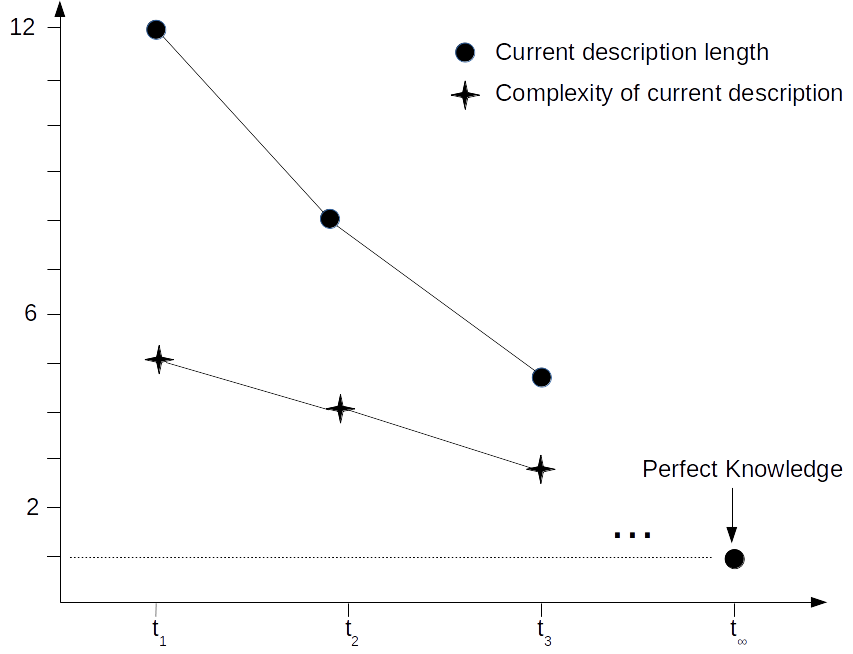
\includegraphics[scale=0.5]{Perfect_Knowledge}
\caption{\label{fig:Perfect_Knowledge}In Pursuit of Perfect Knowledge}
\end{figure}

%
% Section
%

\section{Unknonwn Unknown}

{\color{red} TODO: pending}

Knonw unknown

Unknown unknown

Finally, there exists a last category of unknonw, what we call the unknowable unknown unknown. This category refers to those entities we

Unknowable unknown unknonwn. In this book we are interested in the unknown unknown

%
% Section: Science vs. Pseudoscience
%

\section{Science vs. Pseudoscience}

{\color{red} TODO: Provide a characterization of the difference between science and pseudoscience. In science, nescience decreases with time, in pseudoscience not.}

%
% Section: Nescience of Areas
%

\section{Nescience of Areas}
\label{sec:nescience_areas}

In the same way we studied the properties of individual topics, we could study the properties of areas. An \emph{area} is a subset of topics $A\subset T$. The concept of area is useful as long as all the topics included in the area share a common property. What is exactly that property tehy share depends on the particular set $T$.

\begin{definition}
Given an area $A\subset T$, we define the \emph{average complexity of the area} $C_{A}$ as $C_{A}=\frac{1}{n}\sum_{t\in A}C_{t}$, and the \emph{average nescience of the area} $N_{A}$ as $N_{A}=\frac{1}{n}\sum_{t\in A}N_{t}$, where $n$ is the cardinality of $A$.
\end{definition}

For example, in case of research topics, an area could be a knowledge area, like biology, that will contain all the topics classified under that area. In this way we could compute and compare the complexity (how difficult is to understand) and the nescience (how ignorant we are) of mathematics, physics, biology, social sciences, and other disciplines.

{\color{red} TODO: This definition can only be introduced once we have the concept of best current description.}

An even easier approximation of the concept of redundancy of an area, is based on the average redundancy of the topics that compose that area.

\begin{definition}
Let $A \in \mathcal{T}$ an area, and $d_A$ a description. We define the \emph{average redundancy of the description} $d_A$ as:
\[
\bar{\rho}(d_{\hat{A}}) = \sum
\]
\end{definition}

{\color{red} TODO: Study some properties of this definition}

{\color{red} TODO: How these three definitions releate to each other?}



%
% Section: References
%

\section*{References}

{\color{red} TODO: Add the paper of Chaitin about the Berry paradox}

{\color{red} TODO: That there are numbers that are not computable can be found in the original paper of Turing}

{\color{red} TODO: Perhaps Ii should provide a couple of references in epistemology and ontology}
